% Generated from tex/chapters/ch04/06_構築の管理.tex for the SWEBOK structure tree
\subsubsection{依存関係の管理}

現代のソフトウェアは、多くの外部ライブラリやフレームワークに依存する。Java の Maven、JavaScript の NPM などのパッケージ管理ツールは、依存関係の導入、更新、削除を自動化する。しかし、依存関係は便利である一方、リスクも運ぶ。

依存関係の集合は、供給網のようなネットワークを作る。直接使っているライブラリが、さらに別のライブラリに依存していることも多い。どこかに脆弱性、ライセンス衝突、保守停止、悪意あるコードがあれば、自分の製品にも影響する。

依存関係管理では、不要な依存を避ける、信頼できる依存だけを使う、ライセンスを確認する、脆弱性情報を監視する、バージョン更新を計画する、ロックファイルやソフトウェア部品表を活用する、といった実践が重要である。

\begin{figure}[htbp]
\centering
\IfFileExists{assets/fig-ch04-05.png}{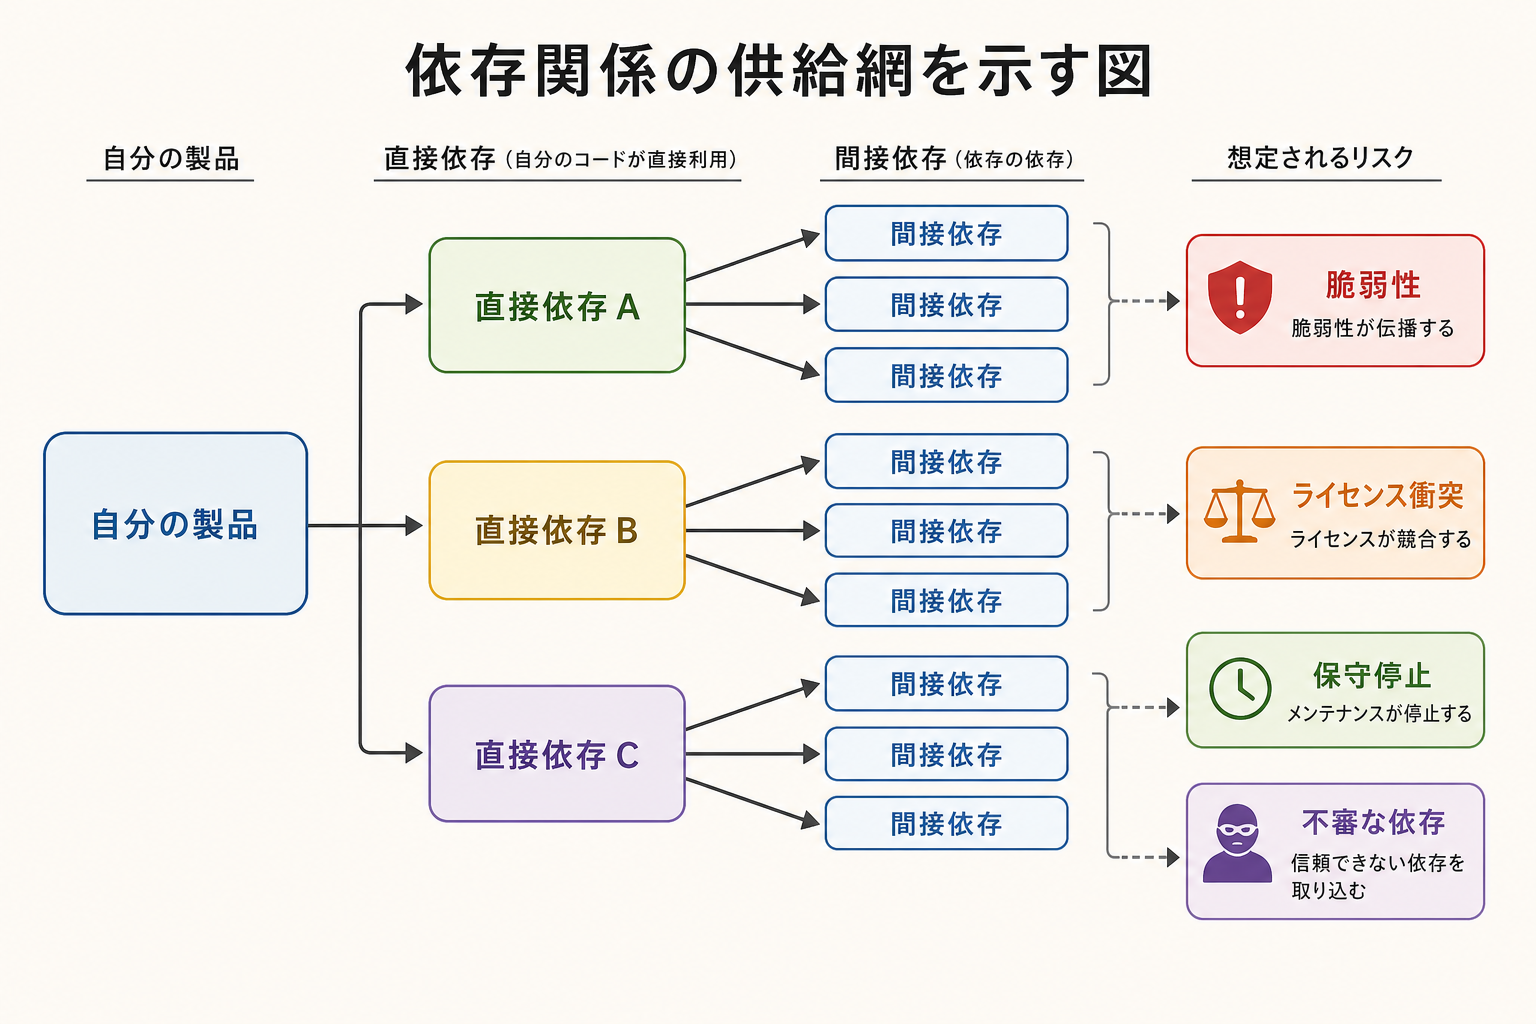
\includegraphics[width=0.96\linewidth]{assets/fig-ch04-05.png}}{\fbox{\parbox[c][48mm][c]{0.9\linewidth}{\centering 画像生成待ち\\依存関係の供給網を示す図}}}
\caption{依存関係の供給網を示す図}
\label{fig:ch04-05}
\end{figure}
